% IEEE Conference paper document class
\documentclass[conference]{IEEEtran}

% code listings
\RequirePackage{listings}
\lstset{
  basicstyle=\ttfamily,
  xleftmargin=36pt,
  xrightmargin=12pt,
  numberstyle=\tiny,              % the size of the fonts that are used for the line-numbers
  numbers=left,                   % where to put the line-numbers
  stepnumber=1,                   % the step between two line-numbers. If it's 1 each line
  tabsize=2,                      % sets default tabsize to 2 spaces
  breaklines=true,                % sets automatic line breaking
  breakatwhitespace=true,         % sets if automatic breaks should only happen at whitespace
  escapeinside={\%*}{*)},         % if you want to add a comment within your code
  showstringspaces=false,         % don't show spaces in strings as little _ style characters
}

% For wrapping text in tables
\usepackage{array}

\usepackage[pdftex]{graphicx}
% declare the path(s) where your graphic files are
\graphicspath{{../thesis/}}

% Support for floats
\RequirePackage{float}

% For more table formatting
\RequirePackage{booktabs}

% Use hyperlinks for convenience, but let's not make them coloured
\RequirePackage[bookmarks,colorlinks,breaklinks]{hyperref}
\hypersetup{
  colorlinks,
  citecolor=black,
  filecolor=black,
  linkcolor=black,
  urlcolor=black
}

% Use the excellent biblatex package with IEEE style, sorted = none makes the numbering appear in order
\RequirePackage[american]{babel}
\RequirePackage{csquotes}
\RequirePackage[
  sorting = none,
  url = false,
  hyperref = true,
  style = ieee,
  bibencoding = utf8]{biblatex}
\DeclareLanguageMapping{american}{american-apa}

% Bibliography
\bibliography{fullrefs}

\begin{document}

\title{Using traffic analysis to identify The Second Generation Onion Router}

\author{
  \IEEEauthorblockN{John Barker}
  \IEEEauthorblockA{
  School of Computer and\\Security Science\\
  Edith Cowan University\\
  Mt Lawley, Western Australia\\
  Email: jebarker@our.ecu.edu.au}
  \and
  \IEEEauthorblockN{Peter Hannay}
  \IEEEauthorblockA{
  School of Computer and\\Security Science\\
  Edith Cowan University\\
  Mt Lawley, Western Australia\\
  Email: p.hannay@ecu.edu.au}
  \and
  \IEEEauthorblockN{Patryk Szewczyk}
  \IEEEauthorblockA{
  School of Computer and\\Security Science\\
  Edith Cowan University\\
  Mt Lawley, Western Australia\\
  Email: p.szewczyk@ecu.edu.au}
}

\maketitle

\begin{abstract}
Anonymous networks provide security for users by obfuscating messages with
encryption and hiding communications amongst cover traffic provided by other
network participants. The traditional goal of academic research into these
networks has been attacks that aim to uncover the identity of network users.
But the success of an anonymous network relies not only on it's technical
capabilities, but on adoption by a large enough user base to provide adequate
cover traffic. If anonymous network nodes can be identified, the users
can be harassed, discouraging participation. Tor is an example of widely used
anonymous network which uses a form of Onion Routing to provide low latency
anonymous communications. This paper demonstrates that traffic from a simulated
Tor network can be distinguished from regular encrypted traffic, suggesting that
real world Tor users may be vulnerable to the same analysis.
\end{abstract}

\section{Introduction}

The first anonymous digital network, commonly known as MixNet was proposed by
\citeauthor{Chaum:1981p296} in \citetitle{Chaum:1981p296}
\parencite{Chaum:1981p296}. This paper introduced a concept integral to many
future anonymity providing designs, an intermediate system responsible for
delivering messages without the identifying details of correspondents. The
intermediate system, referred to as a 'mix' also employed public key
cryptography to ensure that eavesdroppers could not obtain delivery information.

This seminal paper spurred research into new techniques for providing anonymity
and privacy for digital networks. One of these, The Second Generation Onion
Router (Tor) is based on technology originally designed by the U.S. Naval
Research Lab in 1996 \parencite{Goldschlag:1996wy} and enjoys some measure of
popularity, with an average of two hundred thousand active users as of March
2011 \parencite{The-Tor-Project-Inc.:2011fk}.

\section{The Second Generation Onion Router (Tor)}

Like a mix, messages sent over an onion routing network were encrypted with
their routing information and delivered to an intermediate server for forward
delivery.  Unlike the mix however, messages delivered using the onion routing
network were encrypted multiple times, each 'layer' using a different
encryption key and routing instructions. The first node in a chain would only
be able to encrypt the routing instructions to deliver the message to the next
node. Each node in the sequence decrypting a layer until the complete message
is decrypted and transmitted to the destination.

\begin{figure}[H]
  \centering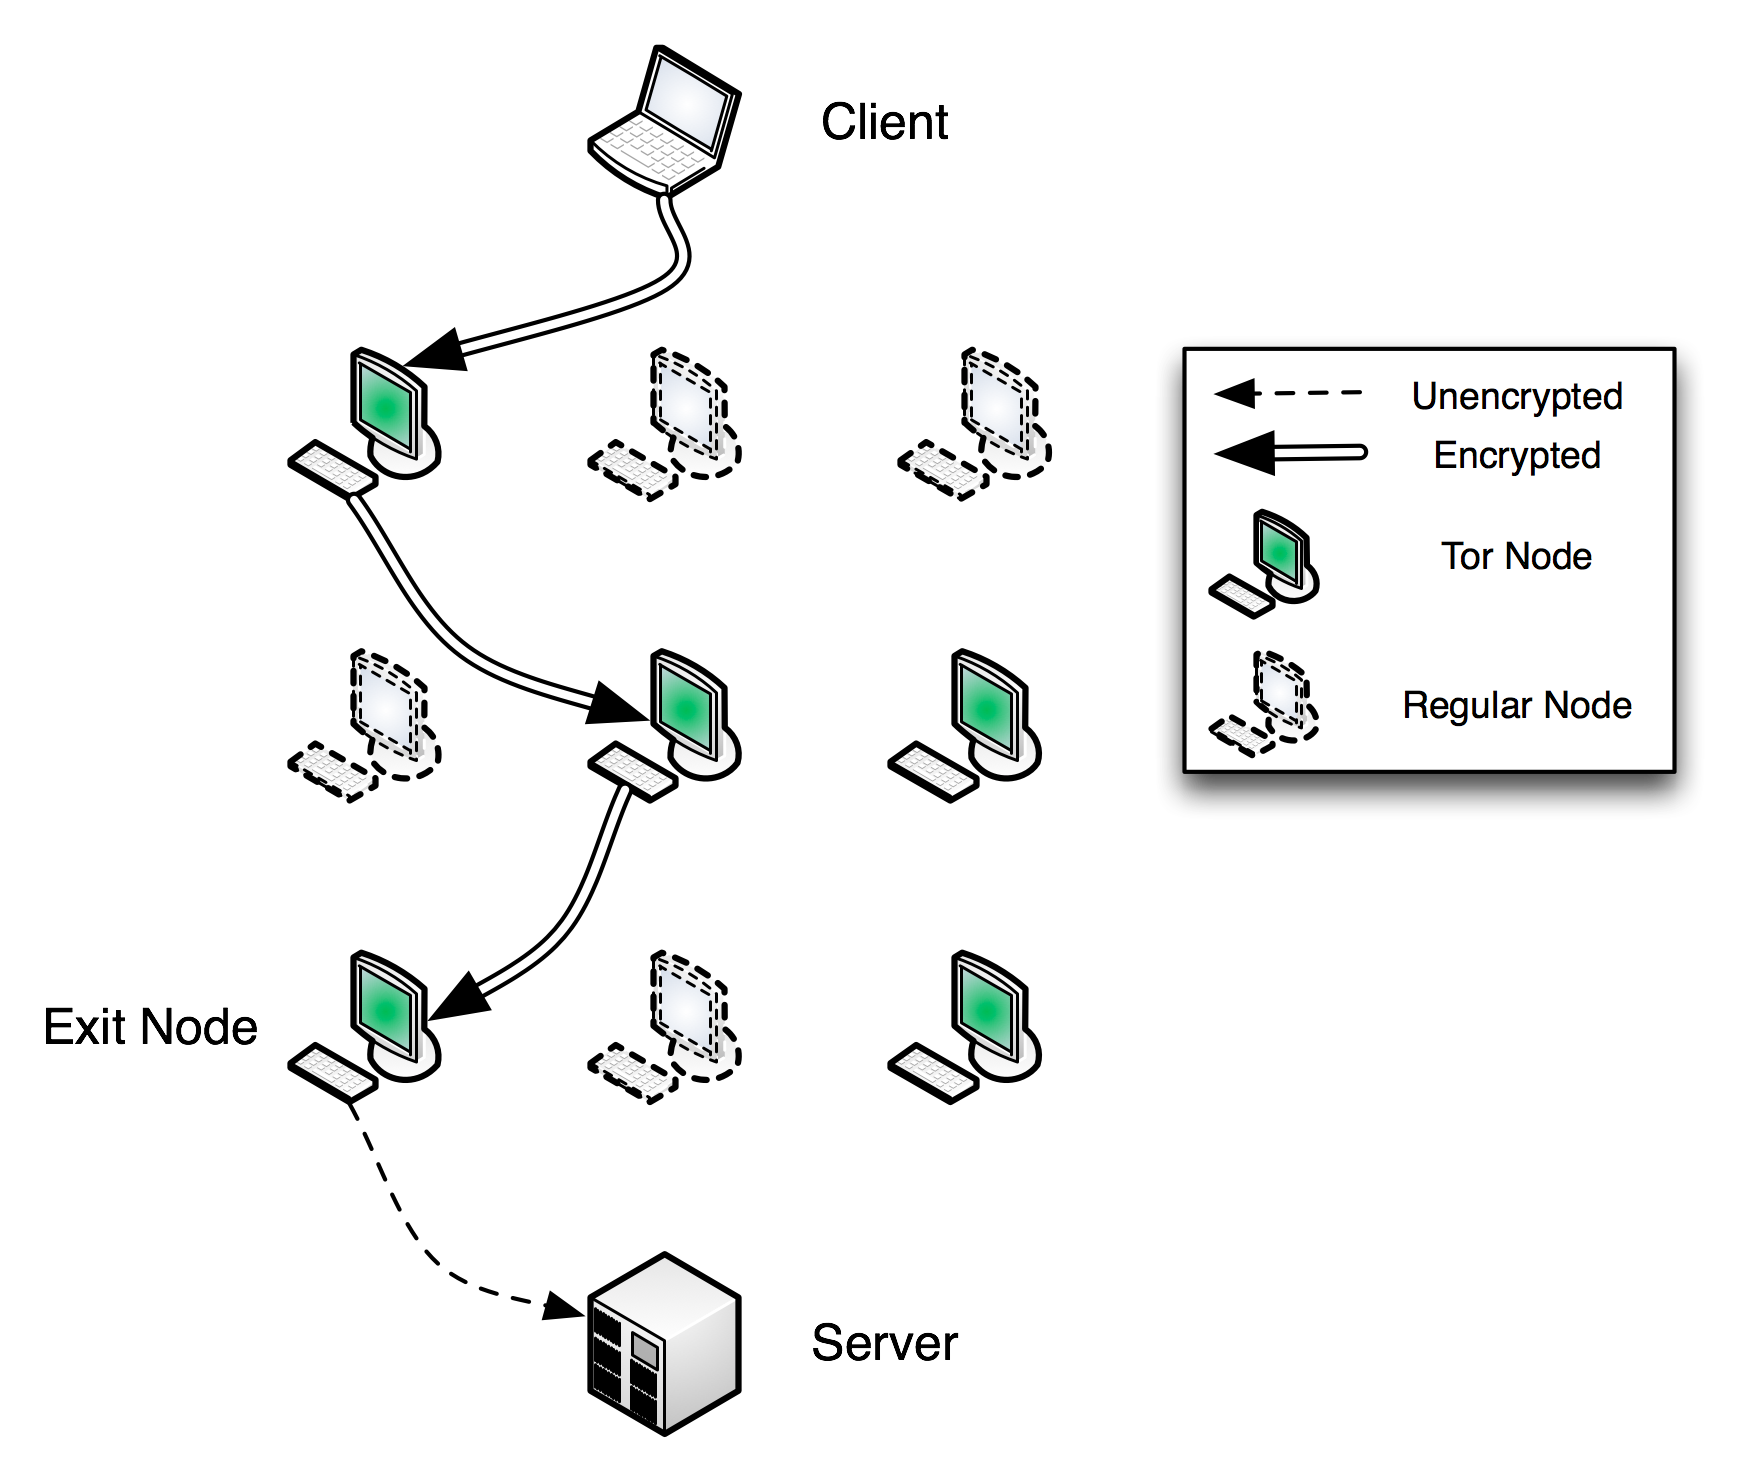
\includegraphics[width=\linewidth]{tor-network-diagram}
  \caption{The Tor Network}
  \label{tor-network}
\end{figure}

Traffic enters the Tor network through an onion proxy which accepts TCP streams.
Some identifying features are scrubbed from the data using application filters
before the data is relayed over the network through TLS \parencite{website:TLS}
encrypted connections. The intermediate nodes responsible for routing messages
are known as relays and are typically chained together to construct a circuit.
When traffic leaves the Tor network it is delivered by a special kind of relay
known as an exit node. At an exit node the data is transmitted in the original
format it was supplied to at the onion proxy.

The onion proxy builds circuits incrementally, first obtaining a session key
from each successive relay in a circuit. Once all session keys for a circuit
have been obtained, the message is broken into fixed sized cells of 512 bytes
and iteratively encrypted using the session key of each node in the circuit in
the reverse order that the data traverses the network. Cells come in two forms:
control cells and relay cells. Control cells are used to create and maintain
circuits, while relay cells contain commands for circuit maintenance and
additional data for verifying message integrity and identifying streams.

\section{Weaknesses and Attacks}

When designing a system such as Tor, a number of trade-offs have to be made
between the strength of the security provided and the convenience and
performance of the system. Tor designers consciously prioritized low latency,
usability and flexibility against security goals such as security against end
to end attacks \parencite[4]{Dingledine:2004p314}. This means that by design,
Tor is vulnerable to a global passive adversary, however there are some attacks
that were not expected by the designers.

A well known attack involves sniffing traffic that leaves exit nodes to
capture private information \parencite{website:tor-password-leak}. Many users
assume that Tor provides end to end encryption, and transmit private information
over the Tor network.

Technologies such as Javascript and Flash can be embedded in web pages accessed
by Tor users, and have control over network resources. By injecting network
traffic with certain patterns alongside regular network traffic, Tor users can
be identified \parencite{Abbott:2007p298}.

Tor bridges, intended as a way to get censored users access to Tor are easily
identified. They are also vulnerable to clogging attacks which make bridge
operators more easily identified \parencite{McLachlan:2009p197}.

\textcite{Murdoch:2005p325} proposes a technique to identify users by estimating
the latency of individual Tor nodes using a hostile Tor node. The hostile Tor
node is able to send data to users using a predictable traffic pattern and
identify this pattern as it is repeated through the network, correlating streams
back to individuals.

This attack was shown to be impractical as the Tor network grew in size, with
the increased number of users adding enough congestion to mask the introduced
identifying patterns \parencite{Evans:2009p315}. However a weakness in the Tor
design meant that particularly configured hostile nodes could amplify the
deliberately introduced congestion to make individuals identifiable on the
larger network.

\section{Significance}

Most conventional attacks against secure networks are known as traffic analysis,
this is the process of examining information about the communications rather
than the information contained within them. This information may include the
size of messages communicated, their frequency and timing. Many researchers have
proposed traffic analysis techniques that allow attackers to reveal the
identities of Tor users.

While Tor has been the subject of much academic literature
\parencite{Hopper:2007p347,Murdoch:2007p320,Herrmann:2009p1189}, the primary
objective of researchers has historically been the attempt to reveal
participant identities \parencite[3]{Murdoch:2005p325}.  Many attack techniques
proposed have been somewhat academic in nature and not necessarily feasible in
practice \parencite{Raccoon:2008fk}. In certain circumstances they require
compromise of large parts of the Tor network, supplying hostile data to Tor
users or complicated knowledge of usage patterns and an excess of patience. The
technique demonstrated in this paper is a low cost technique, which does not
require sophisticated equipment and can be completed by a passive observer.

\section{Traffic Classification}

When considering the use of traffic analysis for classification of Internet
communications, three techniques are used: exact matching, heuristic matching
and machine learning \parencite{Zhang:2009p1188}. Since Tor employs strong
encryption and can communicate on any port, it can easily an exact matching
technique through simple configuration options.

Heuristic based techniques have been designed to classify encrypted
communications, including the identification of P2P traffic
\parencite{Karagiannis:2004p6400,Perenyi:2006p6325,John:2008p1376} and viruses
\parencite{Lazarevic:2003p6450}.

Machine learning algorithms have also been used successfully to classify
encrypted traffic including Skype \parencite{Alshammari:2009p7474} and to
identify application protocols tunnelled over SSH \parencite{Dusi:2008p6254}.
An previous attempt to classify Tor using Bayesian networks was attempted in
\textcite{Herrmann:2009p1189} without great success.

It is difficult to say what machine learning technique is the most effective as
no consensus has been reached, the literature covers a wide variety of
techniques each with vastly different goals and no two techniques can be
directly compared as the data used for analysis has not been disclosed
\parencite{Kim:2007p3867}. However some attempt has been made at comparison in
\textcite{Williams:2006p3849} which suggests that the C4.5 algorithm has the
greatest performance and accuracy when compared to a number of Bayesian
algorithms. \textcite{Mohd:2009p6484} compares thirty machine learning
algorithms to find random tree, IB1, IBK and random forest algorithms
obtaining the greatest classification accuracy.

\section{Experiment}

To determine if Tor traffic can be distinguished from regular encrypted
traffic, an experiment was conducted to generate a series of traces for
comparison. Network traffic was generated using the commonly available Firefox
browser, version 3.6.8 installed on an Ubuntu 10.04 desktop operating system.
One hundred and seventy simulations were run of varied user interactions
against a sample of thirty websites, using version 1.0.6 of the Selenium
Browser testing framework. A private Tor network was configured running three
directory servers and fifteen relays, with version 0.2.1.26.

The experiment consisted of three phases, the first was the capture of regular
HTTPS traffic which began Sunday the 3rd of October 2010 and finished Sunday
the 17th that same month. Phase two began immediately after and continued two
weeks till the 31st of October. This phase involved capturing regular HTTP
traffic routed through a private Tor network. The final phase began on the 7th
of November and concluded on the 21st, this phase was the capture of HTTPS
traffic through a private Tor network.

To reduce the affect of confounding variables, all phases conducted the same
simulations, on an isolated test network and were conducted within a virtual
machine snapshot which was periodically rolled back to a clean, known state.
The experiment yielded three sets of, a summary is included in table
\ref{table:datasets}.

\begin{table}[H]
  \begin{tabular*}{\linewidth}{lrrr}
    \toprule
    Phase & Total Size & Packets & Sessions\\
    \midrule
    HTTPS & 9.52GB & 11,883,703 & 236,659\\
    HTTP over Tor & 10.50GB & 14,823,849 & 168,876\\
    HTTPS over Tor & 5.58GB & 8,161,620 & 95,203\\
    \bottomrule
  \end{tabular*}
  \caption{Captured Data} \label{table:datasets}
\end{table}

\section{Results}

The data captured was in the form of 1MB capture files which were recombined
with mergecap \parencite{Renfro:fk} and processed by NetAI
\parencite{swinbut:2006fk} to produce ARFF format files for use by Weka
\parencite{Hall:2009p7662,Bouckaert:2010we}. NetAI identifies flows inside the
capture files and produces a number of statistics to be used as attributes for
classification.

All of the algorithms chosen were able to successfully classify HTTPS and HTTP
over Tor traffic with accuracy in excess of 90\%, with the Adaboost algorithm
unable to classify HTTPS over Tor. The best performing algorithm random forest
was able to classify HTTP over Tor with 93.7\% accuracy and a false positive
rate of 3.7\%. HTTPS over Tor was more easily identified with a 97.7\% accuracy
and low false positive rate of 0.3\%. A summary of the results obtained by
these machine learning classifiers is available in Table \ref{table:results}.

\begin{table}[H]
  \begin{tabular*}{\linewidth}{lrrr}
    \toprule
    & True Positive Rate & False Positive Rate & ROC Area \\
    \midrule
    \multicolumn{3}{l}{Random Forest}\\
    \midrule
    HTTPS & 0.957 & 0.036 & 0.99\\
    HTTP over Tor & 0.937 & 0.037 & 0.986\\
    HTTPS over Tor & 0.977 & 0.003 & 0.999\\
    Weighted Avg. & 0.954 & 0.03 & 0.99\\
    \midrule
    \multicolumn{3}{l}{j4.8 With 10 fold cross validation}\\
    \midrule
    HTTPS & 0.951 & 0.04 & 0.989\\
    HTTP over Tor & 0.978 & 0.043 & 0.98\\
    HTTPS over Tor & 0.97 & 0.007 & 0.992\\
    Weighted Avg. & 0.964 & 0.018 & 0.986\\
    \midrule
    \multicolumn{3}{l}{Adaboost}\\
    \midrule
    HTTPS & 0.95 & 0.001 & 0.975\\
    HTTP over Tor & 0.999 & 0.324 & 0.838\\
    HTTPS over Tor & 0 & 0 & 0.777\\
    Weighted Avg. & 0.785 & 0.109 & 0.891\\
    \bottomrule
  \end{tabular*}
  \caption{Results from Machine Learning Classifiers} \label{table:results}
\end{table}


With some relative success classifying Tor traffic using unsupervised machine
learning techniques, the captures were examined for a heuristics based
classification approach. When a histogram of packet sizes for each of the
packet traces is produced, a clear distinction can between seen between the
sample sets as seen in Figures \ref{https_hist}, \ref{http_tor_hist} and
\ref{https_tor_hist}.

\begin{figure*}
  \centering\includegraphics[width=0.9\linewidth]{https_hist}
  \caption{Histogram of packet size for HTTPS traffic}
  \label{https_hist}
\end{figure*}

\begin{figure*}
  \centering\includegraphics[width=0.9\linewidth]{http_tor_hist}
  \caption{Histogram of packet size for HTTP traffic over Tor}
  \label{http_tor_hist}
\end{figure*}

\begin{figure*}
  \centering\includegraphics[width=0.9\linewidth]{https_tor_hist}
  \caption{Histogram of packet size for HTTPS traffic over Tor}
  \label{https_tor_hist}
\end{figure*}

Investigating more closely, by examining individual packet traces some
significant patterns begin to appear. Table \ref{table:packet_sizes} shows the
packet sizes seen for the first 6 packets of a 1\% sample of sessions in each
phase of data captured. The first few packets contain 0 bytes of data, these
are the typical SYN, SYN/ACK and ACK flagged packets that are used to initiate
a TCP/IP connection. Following that only two packet sizes are seen for HTTPS
connections. For Tor sessions a range of packet sizes from 131 to 152.

\begin{table}[h]
  \begin{tabular*}{\linewidth}{lp{0.7\linewidth}}
    \toprule
    Index in Stream & Observed Packet Sizes\\
    \midrule
    HTTPS\\
    \midrule
    0 & 0\\
    1 & 0\\
    2 & 0\\
    3 & 100, 110\\
    4 & 0\\
    5 & 122, 516\\
    6 & 0\\
    7 & 6, 139\\
    8 & 0, 6, 37\\
    9 & 0, 37, 459, 465, 471, 514, 515\\
    10 & 0, 37, 417, 418, 419, 429, 436, 438, 439, 447, 448, 449, 454, 459, 463, 464, 465, 466, 470, 471, 486, 497, 499, 512, 513, 514, 523\\
    \midrule
    HTTP Over Tor\\
    \midrule
    0 & 0\\
    1 & 0\\
    2 & 0\\
    3 & 131, 132, 133, 134, 135, 136, 137, 138, 139, 140, 141, 142, 143, 144, 145, 146, 147, 148, 149, 150, 151, 152\\
    4 & 0\\
    5 & 915, 916, 917, 918, 919, 920, 921, 922, 923, 924, 925, 926, 927, 928, 929, 930, 931, 932, 933, 934\\
    6 & 0\\
    7 & 198\\
    8 & 0, 250, 266\\
    9 & 0, 250, 266, 293, 309, 325\\
    10 & 0, 293, 309, 325, 1448\\
    \midrule
    HTTPS Over Tor\\
    \midrule
    0 & 0\\
    1 & 0\\
    2 & 0\\
    3 & 131, 132, 133, 134, 135, 136, 137, 138, 139, 140, 141, 142, 144, 145, 146, 147, 148, 149, 150, 151, 152\\
    4 & 0\\
    5 & 914, 915, 916, 918, 919, 920, 921, 922, 923, 925, 926, 927, 928, 929, 930, 932, 934, 935, 936\\
    6 & 0\\
    7 & 197, 198\\
    8 & 0, 250, 266\\
    9 & 0, 250, 266, 293, 309, 325\\
    10 & 0, 293, 309, 325, 1448\\
    \bottomrule
  \end{tabular*}
  \caption{Packet sizes} \label{table:packet_sizes}
\end{table}


This knowledge can be used to build a rudimentary classification algorithm to
identify Tor traffic, the pseudo code for an example algorithm is included in
Figure \ref{psuedo_matcher}.

\begin{figure}[H]
  \begin{lstlisting}[language=ruby]
    if  packet[3] > 130 and
        packet[3] < 153 and
        packet[5] > 913 and
        packet[5] < 937 then
      is_tor = true
    else
      is_tor = false
    end
  \end{lstlisting}
  \caption{Pseudo Code for Matching a Tor Session}
  \label{psuedo_matcher}
\end{figure}

Applying this algorithm to the complete traces
yields the results as seen in Table \ref{table:heuristic-results}.

\begin{table}[H]
  \begin{tabular*}{\linewidth}{lr}
    \toprule
    Protocol & Identified as Tor\\
    \midrule
    HTTPS & 1.06\%\\
    HTTP over Tor & 98.13\%\\
    HTTPS over Tor & 97.54\%\\
    \bottomrule
  \end{tabular*}
  \caption{Results from Heuristic Classifier}
  \label{table:heuristic-results}
\end{table}

When examining the cases where the algorithm failed to identify Tor streams, in
all cases the session had failed to successfully initiate the handshake
required for a TCP session. Which meant that no meaningful data could have been
transmitted.

\section{Discussion}

Using Tor as a communications proxy incurs some overhead, sufficient enough
that when using a Tor proxy in controlled conditions, its traffic can be
distinguished from regularly encrypted traffic. This overhead may be sufficient
enough that Tor nodes in a real world network can be identified by using
readily available eavesdropping techniques.

The encryption layers that wrap Tor level communications, do not
appear to obfuscate the size of communications sent between Tor nodes. This is
most apparent in the composition of packet sizes that make up an individual
session, with Tor sessions showing a large percentage of packets just large
enough to fit the 512 byte cells that make up the Tor protocol.

However, this experiment was based on a small set of simulated data, with which
it would be impossible to cover all possible real world conditions. The
variability and noise present in the real Tor network may make this
classification technique impossible.


\section{Conclusion}

This research demonstrates that Tor does have characteristics that make it
distinguishable from regular encrypted traffic. The encryption used by Tor does
not appear to blur the size of communication cells sufficiently to prevent
automated identification of Tor traffic, even with only a few observed packets.
While the scope of this research is limited, it suggests that it may be
possible to build simple software to automatically identify Tor users and block
them from the network.

Further research needs to be conducted with live packet traces from real
participants in the Tor network. Most existing traffic classification research
operates this way, using exact matching techniques to separate traces collected
into treatment and control groups. Real Tor traffic might be captured from
publicly available and co-operating Tor nodes and compared to real encrypted
sessions between well known public HTTPS servers.

Training a classifier against real world traffic will account for the different
and varied nature of packet switching hardware, with different maximum
transmission units, performance capabilities and geographic location.

The heuristic based classifier used in this paper used a single attribute: the
size of individual packets in a stream, to classify with great accuracy. But
other attributes may be considered, the most typical of these being inter
packet arrival time - though this is likely to be more affected by natural
variability.

The encrypted traffic generated in the first phase of the experiment, only
covered a single application and version. It may be possible that other
applications use the same protocol with encryption and have characteristics
similar to that produced by Tor. This would lead to any proposed classifier
generating false positives. Further research should also consider the nature
and characteristics of a wider set of encrypted communications.

\printbibliography

\end{document}
